% !TeX encoding = utf8
% !TeX spellcheck = en_GB

\section{Evaluation}

\subsection{Data}
\label{sec:data-sets}
As map data, we use the OpenStreetMap (OSM) project \parencite{OSMF2016}. 
For temperature data we use the hourly air temperature and relative humidity values are originating from the weather station of the German Weather Service (Deutscher Wetterdienste, DWD) in Rheinstetten near Karlsruhe \parencite{DWD2016}. For a finer spatial resolution we use remote sensing data of a thermal scanner flight provided by the Nachbarschaftsverband Karlsruhe (NVK). The data set consists of two scans, recorded in the morning and in the evening of the 26 September 2008. The data are covering an area of  $\SI{25 805}{\meter} \times \SI{39 555}{\meter}$ (EW NS) and have a resolution of $5\,161 \times 7\,911$  pixels. The measured surface temperature is in the range of \SIrange{-1.7}{18.3}{\celsius} (morning and evening). The average surface temperature of the cropped data sets has been \SI{4.18}{\celsius} (morning) respectively \SI{11.24}{\celsius} evening.  


\subsection{Data Preparation}
First, the OSM data set is cropped to the evaluated area. Afterwards, all ways tagged with \verb|highway|, \verb|railway=platform| or \verb|public_transport=platform| are extracted to obtain the road network.

To compute the edge weights as described above in section \ref{sec:edge-weighting} we need to make some assumptions. That's because the weather data that we use lack either an appropriate spatial resolution or the required temporal resolution. We assume that the actual spatial variation of the temperature conforms with the spatial variation of the thermal scans (deviation from the mean value). For the relative humidity, we assume a constant value over the study area. For the temporal variation, we assume that the temporal variation in the examined area corresponds to the temporal variation measure at the weather station. We apply the morning scan to timestamps between  00:00 and 11:59 and the evening scan between 12:00 and 23:59.

We compute the air temperature at time $t\in T$ for the raster cell $c_{ij}$ as follows:
\begin{equation}
\label{eq:derived-temperature}
T_a(t, c_{ij}) = \begin{cases}
T_{a}^{station}(t) + \delta_{ij}^{morning} & \text{if $0 \leq t < 12$,}\\
T_{a}^{station}(t) + \delta_{ij}^{evening} & \text{if $12 \leq t < 24$,}
\end{cases}
\end{equation}
where $T_{a}^{station}(t)$ is the air temperature measured at the weather station at time $t$ and $\delta^{morning}_{ij}$ respectively  $\delta^{evening}_{ij}$ is the deviation of the raster cell $c_{ij}$ from the mean of all raster cells from the morning respectively evening scan.

We compute an approximation of Steadman's heat index with \textcite[77]{Stull2011}. Since the heat index is only defined for an air temperature between \SI{20}{\celsius} and \SI{50}{\celsius} we use the air temperature as a fall-back value. If the air temperature drops in a raster cell below a comfort threshold $T_a^{comfort}$ or $T_{HI}^{comfort}$, then that comfort value will be used, because temperature below this threshold are not considered harmful. 

For the implementation of the routing we used the GraphHopper framework for Java \parencite{GraphHopper2016}.


To find an optimal point in time we used the procedure described in section \ref{sec:find-optimal-time}.  

For the nearby search, we  use a list of selected OSM tags like \verb|shop=supermarket| or \verb|amenity=pharmacy| as a search criteria. We also only consider locations which have opening hours specified (via the \verb|opening_hours| tag). Additionally, only locations which are in a defined radius around the starting point are considered, at this we use the direct distance (“as the crow flies”). To reduce the computation effort a maximum number of results $k$ can be specified.

As optimization algorithm, we use the implementation of Brent's method in the Apache Commons Mathematics Library \parencite{ASF2016} with 10 random start points to reduce the risk that only a local optimum is found.

\subsection{Results}

\subsubsection{Routing}

\begin{table}
	\centering
	\begin{tabular}{lp{9.25cm}lcc}
		\toprule
		& & temperature & heat index \\
		\midrule
		\multicolumn{4}{l}{Reduction of heat exposure (\% of cases) }   \\
		& overall  & \SI{79.70}{\percent} & \SI{80.53}{\percent}  \\
		& more then \SI{5}{\percent} & \SI{42.72}{\percent} & \SI{45.11}{\percent} \\
		& more then \SI{10}{\percent} & \SI{13.81}{\percent} & \SI{16.07}{\percent} \\
		\multicolumn{4}{l}{Reduction of heat exposure}  \\
		& average  & \SI{4.63}{\percent} & \SI{4.69}{\percent}  \\
		& maximum  & \SI{25.97}{\percent} & \SI{26.17 }{\percent}  \\
		\multicolumn{4}{l}{Increase of distance}  \\
		& average & \SI{5.59}{\percent} & \SI{5.76}{\percent}  \\
		\multicolumn{4}{l}{Reduction of relative heat exposure ($w_h / w_d$)}  \\
		& average  & \SI{2.12}{\celsius} & \SI{2.32}{\celsius}  \\
		\bottomrule
	\end{tabular}
	\caption{Overview of the routing results. The values are relative to the shortest route. \label{tab:results-routing}}
\end{table}

\afterpage{
\begin{figure}
	\centering
	\subfigure[map]{
		\label{fig:route-example:map}
		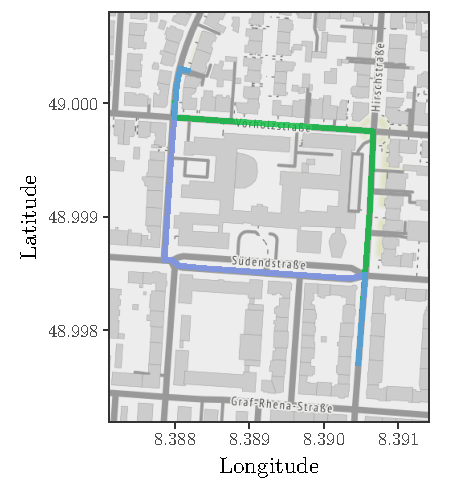
\includegraphics[scale=0.7]{figures/route_example_map}
	}    
	\subfigure[thermal scan (evening)]{
		\label{fig:route-example:raster}
		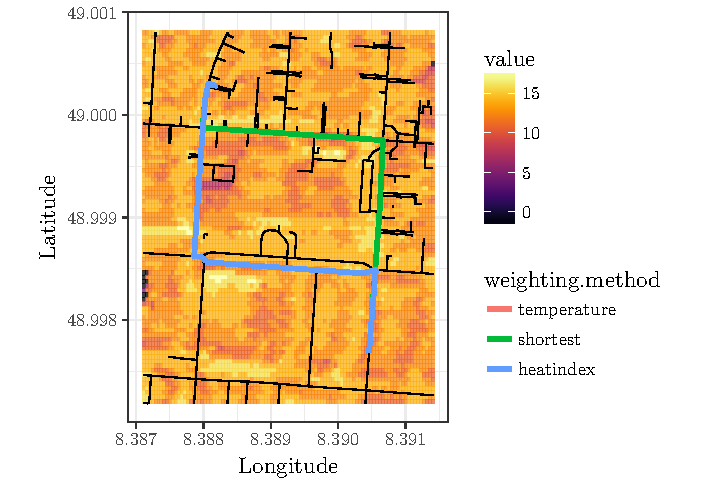
\includegraphics[scale=0.7]{figures/route_example_raster}
	}     
	\caption{Routing example: both the \emph{temperature} and the \emph{heatindex} weighting found the same route. (Map tiles by \textcite{Stamen2017}, under CC BY 3.0\protect\footnotemark{}. Map data by \textcite{OSMF2016}, under ODbL\protect\footnotemark{})}
	\label{fig:route-example}
\end{figure}
\addtocounter{footnote}{-1}
\footnotetext{\url{http://creativecommons.org/licenses/by/3.0}}
\stepcounter{footnote}
\footnotetext{\url{http://www.openstreetmap.org/copyright}}
}

To evaluate the routing, we select 1000 random pairs of start and destinations points form the examined  area and 10 random dates from the period of 1 June to 31 August 2015. For each of the start destination pairs and each date we  perform the evaluation at 7:00, 11:00, 15:00, 19:00 and 23:00, so overall we had $50\,000$ samples. As benchmark we computed for each sample the shortest path. 


An overview of our results is given in table \ref{tab:results-routing}. In many cases the heat exposure could be reduced. On average the heat exposure has been decreased by \SI{\sim 4.7}{\percent} while in the same time the distance was increased by at most \SI{5.76}{\percent} on average. In some cases, the heat exposure can be reduced by up to \SI{25}{\percent}. The weighted average of the thermal comfort measure can be reduced by \SI{\sim 2}{\celsius} on average. There are only slight differences between the air temperature and the heat index as measure for thermal comfort. 

In the example given in figure \ref{fig:route-example} the heat exposure could be reduced by \SI{17.64}{\percent} (\emph{temperature}) and \SI{18.76}{\percent} (\emph{heatindex}), while at the same time the distance only increased by  \SI{0.53}{\percent}.

\subsubsection{Optimal Time}

\begin{table}
	\centering
	\begin{tabular}{lp{9.25cm}lcc}
		\toprule
		& & temperature & heat index \\
		\midrule
		\multicolumn{4}{l}{Reduction of heat exposure}   \\
		& \% of cases  & \SI{68.43}{\percent} & \SI{71.08}{\percent}  \\
		\multicolumn{4}{l}{Reduction of heat exposure}  \\
		& average  & \SI{8.09}{\percent} & \SI{7.73}{\percent}  \\
		& maximum  & \SI{62.29}{\percent} & \SI{62.88}{\percent}  \\
		\multicolumn{4}{l}{Increase of distance}  \\
		& average  & \SI{4.60}{\percent}  & \SI{4.72}{\percent}  \\
		\bottomrule
	\end{tabular}
	\caption{Overview of the results of the combined approach each compared with the reference solution.  \label{tab:results-optimal-time}}
\end{table}

\begin{figure}
	\centering
	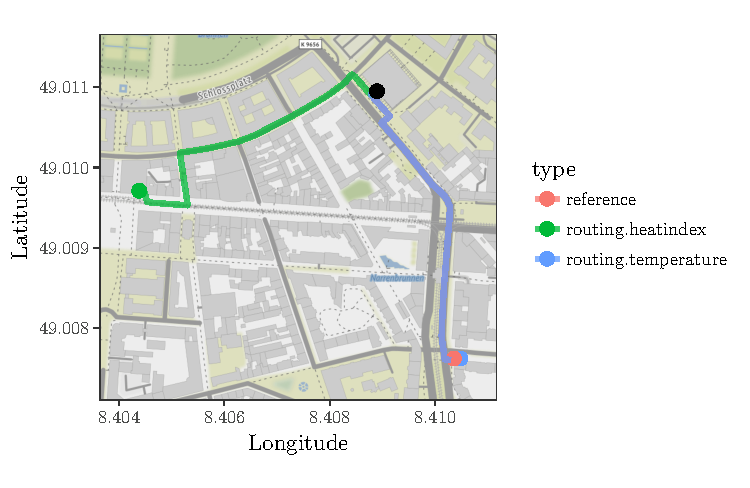
\includegraphics[scale=1]{figures/optimaltime_route_example}
	\caption{Example for nearby search: In the graphic the starting point (black dot) as well as the locations ranked first by the respective method. (Map tiles by \textcite{Stamen2017}, under CC BY 3.0. Map data by \textcite{OSMF2016}, under ODbL)}
	\label{fig:optimaltime-route-example}
\end{figure}

For the evaluation of optimal time finding procedure we selected 750 random start points. One of the following four search criteria has been assigned to each of the start points at random: supermarket, bakery, chemist or pharmacy. For each of the start points a random start time $t_{now}$ has been selected from the period of 8:00 to 20:00. The radius has been set to \SI{1000}{\meter} for all start points and the maximum number of results has been set to 5. Additionally, for all start points a time buffer $t_{buff}$ of 15 minutes has been assumed. 

As a reference solution, we use the closest location found during the nearby search, compute the shortest path from the starting point to this location and evaluated the heat exposure at time $t_{now}$. 

The results for the combined approach are given in table \ref{tab:results-optimal-time}. Here the average reduction compared to the routing approach is significantly higher. This is expected as the heat exposure can vary strongly with the time of the day. 

In the example given in figure \ref{fig:optimaltime-route-example} the \emph{temperature} weighting selected the same pharmacy and optimal point in time (9:27) as the reference solution. Contrary the \emph{heatindex} weighting selected a different pharmacy which is \SI{476.6}{\meter} instead of  \SI{434.5}{\meter} away from the start. Additional the method found a different optimal time (19:39) and those the heat exposure could be reduced by \SI{18.49}{\percent}.  
 
